\chapter{Desarrollo de Simulación de Trayectoria} \label{chp:02_simulacion}

\vspace{0.2cm}

La simulación de trayectoria de un globo sonda es un recurso importante en investigaciones atmosféricas o aeroespaciales, como es el caso de este trabajo, estos simuladores permiten pronosticar y planificar el vuelo de globos, los cuales se basan en modelos matemáticos que describen el comportamiento del  espacio físico donde se desarrolla su trayecto.

\vspace{0.5cm}

En este capítulo se analizan tres modelos físicos matemáticos utilizados en la simulación de trayectoria: modelo atmosférico, modelo geométrico y  modelo dinámico. Cada uno de estos modelos tiene sus propias características y supuestos, que se describen en detalle de forma general y luego de forma específica, además, todos utilizan  el sistema internacional  de unidades.

\newpage

\section{Hipótesis de los modelos} \label{sct:simulacion:hipotesis}

Se describe de forma general los supuestos de la simulación en los diferentes modelos a utilizar; basándose en estos supuestos se identifican y delimita el simulador de trayectoria ascendente y descendente. 

\vspace{0.7cm}

A continuación, los supuestos:

\begin{enumerate}
    \item  El sistema obedece la ley de los gases ideales (ver
anexo \ref{chp:anexo:gases_ideales}), ecuación de la hidrostática (ver anexo \ref{chp:anexo:hidrostatica}) y leyes del movimiento de Newton (mecánica clásica) a lo largo de la trayectoria \cite{libro_dinamica_beer}. 
    \item No existe humedad, radiación solar en la hipotética distribución vertical estratosférica de la trayectoria \cite{isa_1976}. Además, en su distribución vertical la presión interna del globo y externa de la atmósfera se asumen iguales, así mismo la temperatura del globo y la atmósfera. 
    \item Se asume que el sistema emula una partícula de característica esférica con tres grados de libertad, siendo considerada una masa puntual donde interactúan todas las fuerzas que actúan sobre el sistema. Por lo tanto,  por ser un sistema de tres grados de libertad no existen momentos.
    \item  Las componentes horizontales de la velocidad del globo son iguales a las componentes horizontales de la velocidad del viento \cite{lsoda, simulador_chino}, es decir, $\vec{v}_{viento} = \vec{v}_{globo} $ .  Además, se utilizó la convención de meteorología de tener dos componentes de viento U y V, que según su convención la componente U del viento representa el flujo de viento de oeste a este positivo a lo largo de la latitud y la componente V del viento representa el flujo de viento de sur a norte positivo a lo largo de la longitud.
    \item Se toma como premisa que el día y hora del lanzamiento del globo sonda los vientos tiene un comportamiento típico en el proceso de descenso y ascenso. La simulación, en la fecha seleccionada, representa la trayectoria característica que cualquier globo sonda podría experimentar.
\end{enumerate}

\vspace{0.7cm}

La simulación forma parte de modelos estocásticas e hipotéticos de cómo funcionan la distribución vertical de las variables atmosféricas y meteorológicas. Además, no se consideran los modelos térmicos ni elásticos por deformación del globo debido a la duración y enfoque que estos tienen, a diferencias de los zero pressure balloon vistos en subsubsección \ref{tipos_globo} que si es necesario por el tiempo que pasan en la atmósfera que puede ser de unos días, semanas o incluso meses.


\newpage

\section{Datos de entrada e Inicio}

Para la implementación de este trabajo se requiere tener datos de las condiciones iniciales o componentes a utilizar previos a realizar la simulación. En las siguientes subsecciones se detalla esta información antes de  entrar de lleno con los modelos a utilizar.

\subsection{Componentes del Sistema}

La selección de los componentes que se añaden al sistema de globo sonda incluye el paracaídas y el globo mismo, la elección de estos componentes depende de la carga útil que se desea enviar en la misión. Para la simulación, se estima el peso de la carga útil (payload) basándose en el trabajo de graduación realizado por \cite{tesis_estructura_stratoballoon} sobre la estructura. La masa de la carga útil se calcula como 1.769 kg, con un volumen de 517.774 cm³.

Se llevó a cabo una búsqueda para encontrar un globo y un paracaídas comerciales que proporcionen la información requerida por el simulador. Los datos técnicos de estos elementos se muestran en la tabla \ref{tab:globo_datos} y \ref{tab:paracaidas_datos}, respectivamente en \footnote{\textbf{Datos del globo}: \url{https://www.kaymont.com/product-page/hab-1500}} \footnote{\textbf{Datos del paracaídas}: \url{https://the-rocketman.com/recovery-html/}}.

\vspace{0.7cm}
\begin{table}[h]
\centering
\begin{tabular}{ll}
\toprule
        \textbf{Parámetro Globo}                    & \textbf{Valor}  \\
\midrule
        Peso [kg]                  & 1.5    \\
        Diámetro de explosión [m]  & 9.44   \\
        Altitud máxima [m]   & 34,200 \\
        Presión crítica [hPa] & 6.3    \\
\bottomrule
\end{tabular}
\caption{Datos tomados de hoja técnica de Kaymont HAB-1500}
\label{tab:globo_datos}
\end{table}




\vspace{0.7cm}
\begin{table}[h]
\centering

\begin{tabular}{ll}
\toprule
\textbf{Paracaídas}                    & \textbf{Valor}  \\
\midrule
Peso [kg]                 & 0.0992    \\
Diámetro  [m]  & 1.56   \\
\bottomrule
\end{tabular}
\caption{Datos tomados de Rocketman 4ft High Altitude Balloon}
\label{tab:paracaidas_datos}
\end{table}

\newpage

\subsection{Condiciones iniciales y datos de entrada}

Las especificaciones  y la correspondiente información de datos de entrada o valores iniciales del sistema para la simulación de vuelo del globo sonda se presentan en la tabla \ref{tab:datos_start_input}. 

\begin{table}[h]
\centering
\caption{Especificaciones de globo-sonda e información de simulación de vuelo.}
\label{tab:datos_start_input}
\begin{tabular}{cc}
\toprule
              \textbf{Parámetros} &                  \textbf{Valor} \\
\midrule
Fecha y hora de Lanzamiento [UTC] &             2023-06-10 10:00:00 \\
         Objetivo de Altitud  [m] &                           30000 \\
              Base de lanzamiento & Lat: 13.808825, Lon: -89.328988 \\
        Altitud inicial [msnm]    &                             504 \\
                  Masa Globo [kg] &                            1.50 \\
                  Masa Helio [kg] &               0.568913691920873 \\
                Masa Payload [kg] &                            1.77 \\
             Presión Inicial [Pa] &                          101325 \\
          Temperatura Inicial [K] &                          288.15 \\
\bottomrule
\end{tabular}
\end{table}


Es relevante mencionar que el sistema globo sonda parte del reposo cuando es liberado, por lo tanto, su velocidad vertical es cero, solamente siendo afectado por velocidades horizontales por el viento. Además, la fecha y hora elegida no obedece ningún criterio, se hizo de forma arbitraria, pero se asume que se obtiene un comportamiento típico a comparación de otras fechas y horas de lanzamiento.

\subsubsection{Estimación del gas de elevación} \label{ssct:simulacion:gas_y_peso}

La cantidad del gas de elevación es fundamental en la simulación de trayectoria de un globo sonda, ya que permite  obtener la fuerza de empuje que eleva a  la carga útil (payload) y determinar la masa o volumen del gas necesario para llegar a la altitud objetivo o propósito de la misión aeroespacial.  Para desarrollar el cálculo su pudo utilizar dinámica o también aerodinámica con teorías de fluidos, sin embargo, con la intención de reducir la complejidad,  se optó por utilizar  el principio de Arquímedes, la ley de los gases ideales (ver anexo \ref{chp:anexo:gases_ideales}) e hidrostática (ver anexo \ref{chp:anexo:hidrostatica}), modelo estándar atmosférico que se explica más adelante en la sección \ref{sct:simulacion:modelo_atmoferico}  y modelo geométrico que también más se explica posteriormente en la sección \ref{sct:simulacion:modelo_geometrico}. Mayor información de los conceptos que aplican en la estimación según este trabajo en \cite{libro_fisica_giancoli, isa_1976}. 

\newpage

Con respecto a este trabajo, se utiliza el gas helio como gas de elevación\footnote{Existen muchos gases de elevación, los ideales son Hidrógeno y Helio. Lo que los hace gases de elevación es la diferencia de densidad respecto al aire, que es menor. Se prefiere Helio debido a que es más seguro su manejo y es un gas inerte.},  una vez seleccionado el gas se partió de la ecuación de los gases ideales (ver anexo \ref{chp:anexo:gases_ideales})  haciendo una comparación de un estado inicial del gas a un estado final  en el cual existe conservación de masa lo cual es algo lógico porque la masa del gas es constante en todo la trayectoria hasta la explosión del globo en la altitud objetivo asumiendo que no existan fugas del mismo, véase tabla \ref{tab:datos_start_input} altitud objetivo.  Con la anterior comparación del gas en sus estados final e inicial se tiene entonces la ley de los gases de esta forma: 


\begin{equation}
    \label{eq:masa_helio}
    \frac{P_{1} V_{1}}{ T_{1} } = \frac{P_{2} V_{2}}{ T_{2} }
\end{equation}


Donde en ecuación \ref{eq:masa_helio}, el subíndice 1 significa estado del gas en el punto de lanzamiento, punto 1; y subíndice 2 como el punto final al cual la sonda debe de alcanzar, punto 2. En ambos subíndices se conocen el valor de las variables del gas de ecuación \ref{eq:masa_helio} por el estándar  atmosférico \cite{isa_1976}

\textbf{En el punto 1} se conoce la presión y temperatura ($P_{1}$ y $T_{1}$), se desea conocer el volumen inicial o volumen de llenado del globo ($V_{1}$).

\textbf{En el punto 2} conocemos la presión, volumen y temperatura final ($P_{2}$, $V_{2}$ y $T_{2}$ respectivamente), además se toma en cuenta lo expuesto por la hoja técnica que puede soportar el globo seleccionado, ver tabla \ref{tab:paracaidas_datos}. 

Una vez calculada volumen inicial ($V_{1}$) se debe de despejar de la ecuación de la ley de los gases ideales ($PV = nRT$) para calcular la masa, además al resolver todo lo anterior explicado se pudo obtener el volumen inicial y diámetro inicial del globo como también su masa de llenado de helio. En el código de Python desarrollado se utilizó el módulo sympy\footnote{Más información de sympy: \url{https://www.sympy.org/en/index.html}} para resolver las diferentes ecuaciones. 

\textbf{Soluciones alternativas}

Existe otras formas de calcular la cantidad de Helio o gas de elevación utiliza, por ejemplo  en \cite{spain_simulador} se calcula primero el radio de lanzamiento del globo y  luego se obtiene el volumen, para por último hacer una formulación de la ecuación de ley de los gases ideales y obtener la masa del helio además de una comparación si existe flotabilidad. Además, se puede calcular usando dinámica \cite{libro_dinamica_beer},  dimensionando la fuerza de arrastre y fuerza de empuje, teniendo el sistema en reposo donde $\sum F = 0$  como lo indica \cite{lsoda, helio_estimatcion} . Se prefirió la forma mostrada en ecuación \ref{eq:masa_helio} debido a que así se tiene control de la altura objetivo a la cual se desea enviar y se reduce complejidad en el cálculo. 

\newpage

\section{Sistema de Coordenadas}

En figura \ref{fig:crs} se muestran la relación que pueden existir entre diferentes sistemas de coordenadas\footnote{ \href{https://commons.wikimedia.org/wiki/File:International_Standard_Atmosphere.svg}{ CC BY-SA 4.0, autor: Chuckage.  Shows the ECEF coordinates (x, y, z) of a point on the surface of a spheroid.} Sin modificación }. En este caso un cartesiano con un elipsoide de referencia y uno de coordenadas esféricas, los cuales pueden expresar el comportamiento de cualquier sistema que se desplace en el planeta tierra.

\begin{figure}[h]
    \centering
    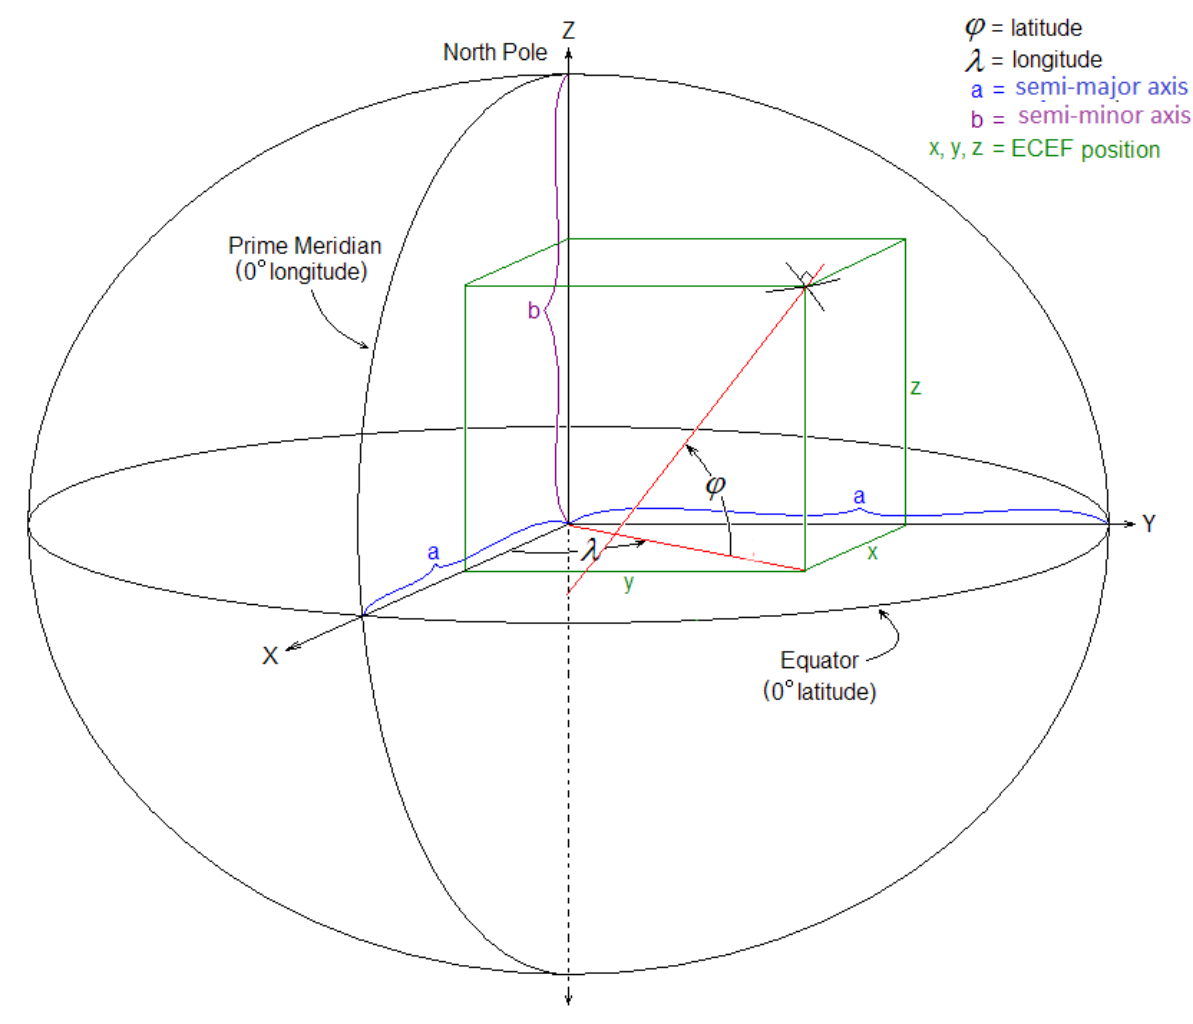
\includegraphics[scale=0.25]{document/figures/02_ECEF_coordinates.png}
    \caption{Sistema de coordenadas}
    \label{fig:crs}
\end{figure}
Por otro lado, en la simulación a desarrollar el movimiento espacial se ha caracterizado en  dos tipos:  vertical y horizontal. Dado el carácter que las distancias son cortas, la curva tierra no es apreciable, así que en su área de operación del globo sonda se trabaja como dos ambientes separados en el cual la vertical se moverá siguiendo la altitud en la que se encuentre en la tierra; por otro lado, en la horizontal, se analiza el problema como proyecciones de EPSG:4326 debido a que son las forma en que entrega la información los GPS en latitud y longitud (WGS84) \cite{libro_gnss},  y por otro lado, EPSG:3857 debido a que es la presentación renderizada de mapas como Google Maps \cite{google_maps}, OpenStreetMap, etc. La decisión está determinada por usar EPSG:4326 y EPSG:3857 para respectivamente tener grados y en la otra proyección usar metros así como están planteadas las ecuaciones diferenciales \ref{eq:viento_x} y \ref{eq:viento_y}, también esta decisión permite el uso de mapas.
 
\newpage

\section{Modelo Atmosférico} \label{sct:simulacion:modelo_atmoferico} 

Se utiliza la  ISA (International Standard Atmosphere) de 1976 \cite{isa_1976} para predecir las condiciones atmosféricas a diferentes altitudes, este modelo proporciona una referencia estándar, invariante e hipotética de la distribución vertical de la temperatura, presión y densidad en función de las diferentes capas de la atmósfera en todo el mundo.  

Además, se incluye información sobre la gravedad que son factores importantes en la trayectoria del globo sonda hasta altitudes estratosféricas. En figura \ref{fig:generalidad_ISA} \footnote{ \href{https://commons.wikimedia.org/wiki/File:International_Standard_Atmosphere.svg}{CC BY-SA 3.0, autor: Cmglee. Derivado de Comparison International Standard Atmosphere space diving.svg.} Sin modificación} se muestra una idea general de la distribución vertical según las diferentes capas de la atmósfera.

\begin{figure}[h]
    \centering
    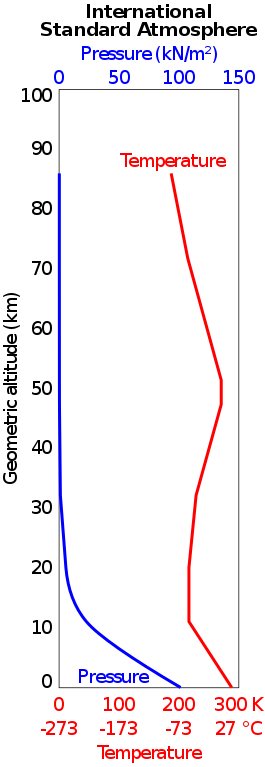
\includegraphics[scale=0.45]{document/figures/02_International_Standard_Atmosphere.png}
    \caption{Comportamiento de las variables  atmosféricas, temperatura y presión en las diferentes capas según ISA.}
    \label{fig:generalidad_ISA}
\end{figure}


\subsection{Gravedad}

La gravedad se hace más débil a medida que se aleja de la masa terrestre, es decir, no es constante a medida que se asciende, sino que disminuye en función de la altitud; esta formulación es proveída por la Ley del Inverso cuadrado  \cite{isa_1976}. Esta disminución se puede expresar de:

\begin{equation}
    \label{eq:gravedad}
    g = g_0 \left(\frac{R_e}{R_e + Z}\right)^2
\end{equation}

\textbf{Donde:}
\begin{itemize}
    \item 	$g_{0}$ es la aceleración estándar debida a la gravedad sobre el nivel del mar, con un valor de $ 9.80665 $  $ m/s^{2} $.
    \item 	$R_e$ es el radio promedio de la Tierra, con un valor de 6,371,000 m.
    \item 	$Z$ es la altitud sobre la superficie de la Tierra.
\end{itemize}

\subsection{Temperatura, presión y densidad} \label{ssct:simulacion:ISA_variables}

Debido a la naturaleza de los globos sonda se presenta un resumen de las capas estratosféricas a las cuales en su trayectoria se podría mover el globo sonda, en tabla \ref{tab:constantes_ISA}  y  \ref{tab:formulas_ISA}  se exponen respectivamente las constantes y ecuaciones matemáticas de las variables temperatura, presión y densidad del modelo atmosférico \cite{tabla_isa}.

% Tabla de las Constantes  ISA (temperatura, presión y densidad).
\begin{table}[ht]
\centering
\begin{tabular}{ccccc}
\hline
\textbf{Capa} & \textbf{$z_0$ [m]} & \textbf{$T_0$ [K]} & \textbf{$\lambda_0$ [K/m]} & \textbf{$P_0$ [Pa]} \\
\hline
1 & 0 & 288.15 & -0.0065 & 101,325.00 \\
2 & 11,019 & 216.65 & - & 22,632.10 \\
3 & 20,063 & 216.65 & 0.0010 & 5,474.89 \\
4 & 32,162 & 228.65 & 0.0028 & 868.02 \\
5 & 47,359 & 270.65 & - & 110.91 \\
\hline
\end{tabular}
\caption{Constantes de la ISA}
\label{tab:constantes_ISA}
\end{table}

% Tabla de las Ecuaciones ISA (temperatura, presión y densidad).

\begin{table}[ht]
\centering

\begin{tabular}{cccc}
\hline
\textbf{Capa} & \textbf{Temperatura [K]} & \textbf{Presión [Pa]} & \textbf{Densidad [kg/m$^3$]} \\
\hline
1 & $T_0 + \lambda_0 (z - z_0)$ & $P_0 \; \left( \frac{T_0}{T} \right)^{g(z) M_{air} / (R_{s} \lambda_0)}$ & $ P / (T \; R_{s})$ \\
2 & $T_0$ & $P_0 \; e^{-g(z) M_{air} (z - z_0) / (R_{s} T)}$ & $ P / (T \; R_{s})$ \\
3 & $T_0 + \lambda_0 (z - z_0)$ & $P_0 \; \left( \frac{T_0}{T} \right)^{g(z) M_{air} / (R_{s} \lambda_0)}$ & $ P / (T \; R_{s})$ \\
4 & $T_0 + \lambda_0 (z - z_0)$ & $P_0 \; \left( \frac{T_0}{T} \right)^{g(z) M_{air} / (R_{s} \lambda_0)}$ & $ P / (T \; R_{s})$ \\
5 & $T_0$ & $P_0 \; e^{-g(z) M_{air} (z - z_0) / (R_{s} T)}$ & $ P / (T \; R_{s})$ \\
\hline
\end{tabular}
\caption{Fórmulas de la ISA}
\label{tab:formulas_ISA}
\end{table}


\newpage

\section{Modelo Geométrico} \label{sct:simulacion:modelo_geometrico}

A medida el globo sonda asciende, el aire se volverá menos denso y el gas en su interior se expandirá por tal motivo, lo que provocará que la geometría del globo cambien,  para calcular tal fenómeno se aplica la Ley de los Gases ideales, la ISA y geometría. Entonces,  con lo anterior y dejando la ecuación en función de la altitud, se tiene:


\begin{equation}
    \label{eq:geometria}
    P(z) \; V = n \; R \; T(z) 
\end{equation}


Donde $ P(z) $ es la presión interna del gas, que será igual a la presión externa atmosférica;  $ n $ es la cantidad de moles del gas de elevación (helio) y $ T(z) $ la temperatura atmosférica igual que la temperatura del gas, por último $ R $ es la constante de los gases ideales.  Se ha asumido que el globo tiene forma esférica,  se  tiene que $r(z)$ como indica\cite{ascentRate_weatherBallon} es:

\begin{equation}
    \label{eq:radio}
    r(z) = \sqrt[3]{\frac{ 3 \; m \; R \; T }{ 4 \pi \; P \; M }}   
\end{equation}
 
La ecuación \ref{eq:radio} se utiliza para determinar tanto en área como en volumen del globo, como se indica en los siguientes apartados. Como dato de entrada para aplicar esta ecuación, es necesario conocer la masa del helio con la cual fue llenado el globo sonda como se indicó en subsubsección \ref{ssct:simulacion:gas_y_peso}.

\subsection{Área transversal}

El área transversal de una esfera es la superficie de corte de una esfera por un plano perpendicular a su eje. En el caso de una esfera perfecta, la sección transversal será un círculo con un diámetro igual al diámetro de la esfera. Por lo tanto, se tiene que:

\begin{equation}
    \label{eq:area_transversal}
    A = \pi r^{2}   
\end{equation}

\subsection{Volumen}
El volumen a medida asciende se puede calcular a partir del volumen de una esfera así:

\begin{equation}
    \label{eq:volumen}
    V  = \frac{4}{3} \pi r^{3}
\end{equation}

\newpage

\section{Modelo Dinámico} \label{sct:simulacion:modelo_dinamico}

Las ecuaciones del movimiento están presenta durante su trayectoria ascendente y descendente \cite{libro_fisica_giancoli, libro_dinamica_beer}, y en ellas es fundamental considerar factores como el viento, la fuerza de arrastre y la fuerza de sustentación para poder predecir la trayectoria del globo con la mayor precisión posible, todo lo anterior se analiza en función del tiempo y posición. Además, este modelo se sustenta con los modelos geométricos y atmosféricos expuestos con anterioridad.

El movimiento de un cuerpo hipotético, como lo descrito en sección \ref{sct:simulacion:hipotesis}, se expresa mediante estas ecuaciones:

\begin{align}
    \displaystyle \sum \vec{F} &= m \; \vec{a}  \label{eq:fuerzas}
    \\
    \displaystyle \sum \vec{M} &= 0 \label{eq:momentos}
\end{align}

Tomando de referencias las ecuaciones \ref{eq:fuerzas} y \ref{eq:momentos}, y al contexto de los globos sonda se desarrolla un sistema de ecuaciones de ascenso y descenso, que representaría el movimiento vertical; además se tendría que desarrollar un sistema de ecuaciones de movimiento horizontal. En las siguientes subsecciones se muestra las ecuaciones del movimiento de la trayectoria del globo sonda.

\begin{figure}[h]
    \centering
    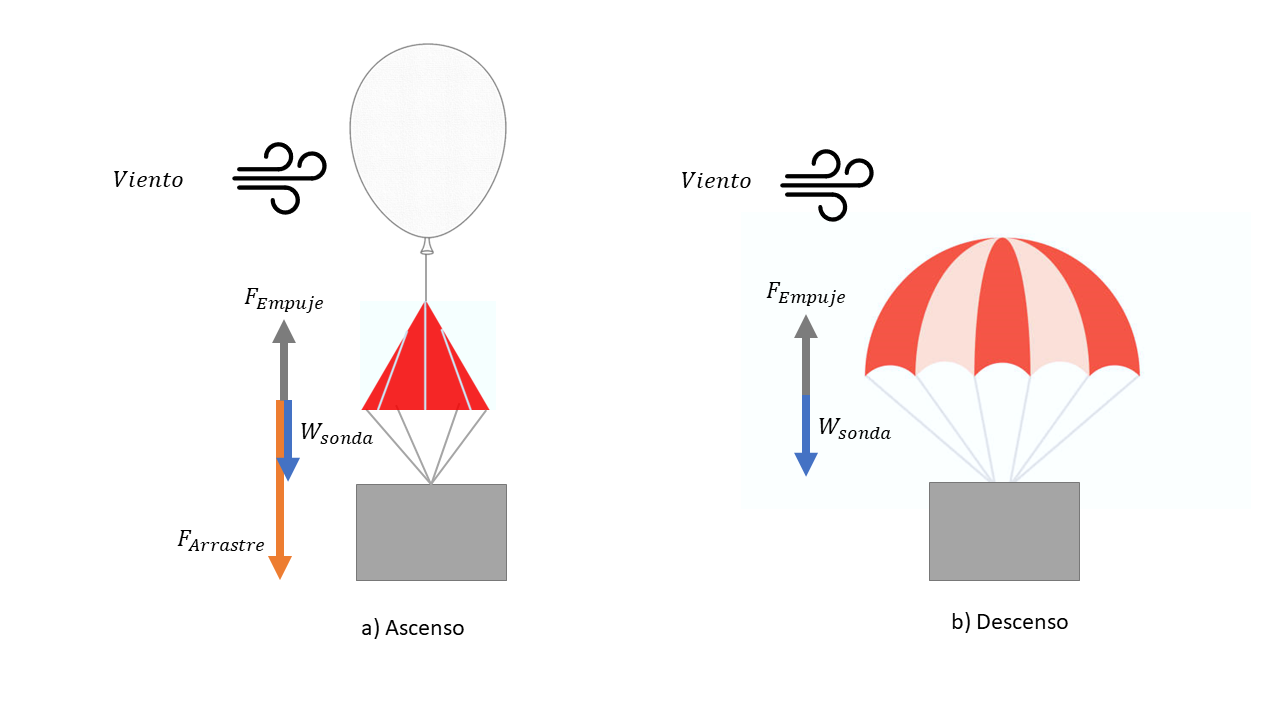
\includegraphics[width=0.75\linewidth]{document/figures/02_DCL_movimiento.png}
    \caption{Diagrama de cuerpo libre del sistema}
    \label{fig:dlc}
\end{figure}

\newpage

\subsection{Ecuación de movimiento vertical}

El movimiento vertical estará compuesto, por una parte, ascendente y una descendente, el cual en el primer instante representa cuando el globo está inflado y aún no ha explotado, el segundo  representa  donde todo el sistema comienza a caer en caída libre atado de un paracaídas. En figura \ref{fig:dlc} se muestra de forma representativa las fuerzas que actúan sobre el globo sonda.

\subsubsection{Ascenso}

Partiendo de un diagrama de cuerpo libre de figura \ref{fig:dlc} con un marco de referencia de un plano cartesiano tradicional,  en el cual se tiene las fuerzas que actúan sobre el globo sonda, se tendría que: existiría una peso $W_{Sonda}$ el cual actuaría negativo, una fuerza de empuje $F_{Empuje}$ encargada de que el globo ascienda y una fuerza resistiva de arrastre $F_{Arrastre}$ , generalizando  se tiene la siguiente ecuación:

\begin{equation}
    \label{eq:newton_ascenso}
  m \frac{\mathrm{d^2} z }{\mathrm{d} t^2}  =  F_{Empuje} - W_{Sonda} - F_{Arrastre}
\end{equation}

De este modo, contextualizando en ecuación \ref{eq:newton_ascenso}  con los modelos anteriores desarrollados y bibliografía consultada \cite{lsoda, ascenso_formula, ascenso_formula_2, constante_CD_y_formula_ascenso, simulador_chino}, se tiene:
\begin{equation}
    \label{eq:ascenso}
     ( m_{b} + m_{gas} + m_{pl} ) \; \frac{\mathrm{d^2} z }{\mathrm{d} t^2}  =  \rho_{atm} (z) \; V_{b} \; g (z) -( m_{b} + m_{pl} ) \; g(z) - \frac{1}{2} C_{D} \; \rho_{atm} \; S_{b} \; \left ( \frac{\mathrm{d} z }{\mathrm{d} t} \right )^{2}
\end{equation}
\textbf{Donde:}
\begin{itemize}
    \item $m_{b}$ es la masa del globo.
    \item $m_{gas}$ la masa del helio en el interior del globo.
    \item $m_{pl}$ es la masa de la carga útil o payload.
    \item $\rho_{atm}$ densidad atmosférica dada por la ISA, ver subsección \ref{ssct:simulacion:ISA_variables}.
    \item  $V_{b}$ volume del globo.
    \item $g$ es gravedad en función de la altitud, ver ecuación \ref{eq:gravedad}.
    \item $C_{D}$ y $S_{b}$  son el coeficiente de arrastre de una esfera y área transversal del globo.
\end{itemize}

En ecuación \ref{eq:ascenso} se comienza describiendo del lado izquierdo de la ecuación las diferentes masas que actúan en el sistema (masa del globo, masa del gas de elevación y masa del payload o carga útil respectivamente), luego de ello se tiene la presión, el volumen que se sustituye por ecuaciones de tabla \ref{tab:formulas_ISA} y ecuación  \ref{eq:volumen}, el  área que se sustituye por ecuación \ref{eq:area_transversal}. Además, se tiene la gravedad, coeficiente de arrastre y velocidad.

Como se hipotetiza que el globo sonda tiene una geometría esférica, el coeficiente de arrastre conocido que oscila entre $10^{4} $  y $10^{5}$ números de Reynolds \cite{constante_CD_y_formula_ascenso, Constatntes_CD_HAB}, por consiguiente en este trabajo se utiliza $C_{D} = 0.47$. 
 

\subsubsection{Descenso}

Una vez el globo llegó a su altura objetivo, este sufrirá una explosión la cual será afectada por la atracción gravitacional de la tierra, lo que hará que descienda en caída libre \cite{modelo_free_falling, redbull_free_falling}, este fenómeno se modela de la siguiente forma:
\begin{equation}
    \label{eq:newton_descenso}
  m \frac{\mathrm{d^2} z }{\mathrm{d} t^2}  =  F_{Arrastre} -W_{Sonda}
\end{equation}
Aplicando los modelos anteriores en ecuación \ref{eq:newton_descenso}, e ingresando los datos de entrada del paracaídas, tenemos que:

\begin{equation}
    \label{eq:descenso}
     ( m_{b} + m_{pl} ) \; \frac{\mathrm{d^2} z }{\mathrm{d} t^2}  =   \frac{1}{2} C_{D} \; \rho_{atm} \; S_{p} \; \left ( \frac{\mathrm{d} z }{\mathrm{d} t} \right )^{2} -( m_{b} + m_{pl} ) \; g(z) 
\end{equation}
\textbf{Donde:}
\begin{itemize}
    \item $m_{b}$ es la masa del globo.
    \item $m_{pl}$ es la masa de la carga útil o payload.
    \item $\rho_{atm}$ densidad atmosférica dada por la ISA, ver subsección \ref{ssct:simulacion:ISA_variables}. 
    \item $C_{D}$ y $S_{p}$  son el coeficiente de arrastre  y área transversal del paracaídas.
    \item     $g$ es gravedad en función de la altitud, ver ecuación \ref{eq:gravedad}.
\end{itemize}

En ecauación \ref{eq:descenso},  la fuerza de arrastre experimentada en el descenso es debido a la acción del paracaídas, y es positiva debido a que marco de referencia optado. La constante de arrastre $C_{D}$ oscila entre 0.5  y  0.8 según \cite{Constatntes_CD_HAB}, en este trabajo se utiliza $C_{D} = 0.8$, además que este dato no es proporcionado por el fabricante del paracaídas. 

\subsection{Ecuación de movimiento horizontal}

El movimiento horizontal es afectado por el viento  en el ascenso y descenso según la altura que se encuentre, ver figura \ref{fig:dlc}, para ello se toma los datos brindados por la National Oceanic and Atmospheric Administration (NOAA). Los datos proporcionados por la NOAA son discretos y están referenciados a alturas fijas, es por ello que es necesario una interpolación para obtener una función que nos permita conocer las condiciones del viento a diferentes alturas. Se trabaja con las siguientes ecuaciones basándose en \cite{lsoda}

\begin{equation}
    \label{eq:viento_x}
    \frac{\mathrm{d} x }{\mathrm{d} t} = - w(z) \cdot  \cos(\phi(z)) = u
\end{equation}

\begin{equation}
    \label{eq:viento_y}
    \frac{\mathrm{d} y }{\mathrm{d} t} = - w(z) \cdot \sin(\phi(z)) = v
\end{equation}

En este apartado, se utilizó el módulo getgfs  de Python \footnote{Más información de getgfs: \url{https://getgfs.readthedocs.io/en/latest/}}, que toma datos del modelo numérico de predicción Global Forecast System (GFS) desarrollado por la NOAA para obtener datos meteorológicos. Este módulo devuelve la interpolación de las componentes  U y V del viento. Al utilizar este módulo,  se elimina el desarrollo de las matemáticas trigonométricas en ecuaciones \ref{eq:viento_x} y \ref{eq:viento_y}, lo que permite realizar la integración de las ecuaciones diferenciales directamente.

Es relevante señalar que las componentes del viento $u$ y $v$ es el formato común en el cual se entregan  los datos del viento en meteorología\cite{lsoda}, a partir de ello se puede calcular la magnitud y dirección del viento. 
 
\section{Funcionamiento y resultados}

Se utilizó Jupyter Notebooks con Python para desarrollar el simulador de trayectoria ascendente y descendente, en el cual se ingresaron todos los datos iniciales y de entrada, luego se desarrolló cada modelo de forma individual para finalizar resolviendo las ecuaciones diferenciales \ref{eq:ascenso}, \ref{eq:descenso}, \ref{eq:viento_x}  y \ref{eq:viento_y}, utilizando la función de Scipy  solve\_ivp(). Dentro de esta función se utilizó el método de integración  "LSODA"  debido a los buenos resultados que se obtiene tal como lo indica \cite{lsoda}; las ecuaciones diferenciales son de segundo orden, fue necesario aplicar una reducción de orden para obtener las soluciones debido a que Python no posee una forma directa para resolverlas.  Además,  en las ecuaciones \ref{eq:viento_x} y \ref{eq:viento_y} se utiliza el módulo de Python pyproj para homogeneizar las unidades  de la superficie de la tierra sobre un plano, transformando la latitud y la longitud de su representación decimal mostrada en tabla \ref{tab:datos_start_input} a unidades de metros.

Una vez realizada la resolución matemática, se obtuvo datos de posición y tiempo del sistema, se sustituyeron en los modelos y ecuaciones pertinentes, recalculándolos debido a que la función solve\_ivp() no devuelve estos valores, y así se obtuvo los datos correspondientes en cada instante y posición como son la presión, temperatura, diámetro del globo, etc.  

\newpage
Por lo anterior,  el simulador representa el comportamiento de la trayectoria descendente y ascendente. Véase las siguientes tablas \ref{tab:ascenso_frag_datos_generados} y \ref{tab:descenso_frag_datos_generados} que contiene una muestra de los datos generados del simulador, estas tablas fueron creadas a partir de almacenar los datos en archivos .csv\footnote{Los archivos .csv se pueden consultar visitando los anexos \ref{chp:anexo:source_thesis}}, que son la base de donde se hace los análisis en el siguiente capítulo.

\vspace{1 cm}

\textbf{Nota:} el código fuente desarrollado para la simulación de trayectoria  se detalla en el anexo \ref{chp:anexo:source_thesis}. Además, es accesible lo realizado en capítulo \ref{chp:03_eda} y toda la documentación perteneciente a este trabajo \footnote{Consulte rápidamente el código fuente, en la siguiente URL: \url{https://github.com/osminlab/Proyec_Gda_Simula_PCB_Nav}}.

% ------------------------------------------------------------------
% Framento de simulación en tablas, con contenido rotado
% ------------------------------------------------------------------

\begin{landscape}
    % TABLA ASCENSO
    \begin{table}
\small
\centering
\caption{Ascenso, fragmento de los datos generados en simulación.}
\label{tab:ascenso_frag_datos_generados}
\begin{tabular}{cccccccccccc}
\toprule
\textbf{t [s]} & \textbf{Lat. ($\phi$)} & \textbf{Long. ($\lambda$)} & \textbf{Alt. (z) [km]} & \textbf{$dz/dt$ [m/s]} & \textbf{u [m/s]} & \textbf{v [m/s]} & \textbf{T [°C]} & \textbf{P [hPa]} & \textbf{$\rho$ [kg/m³]} & \textbf{g [m/s²]} & \textbf{d [m]} \\
\midrule
             0 &                13.8088 &                    -89.329 &                    0.5 &                    0.0 &              0.0 &              0.4 &            11.7 &            954.2 &                     1.2 &               9.8 &            1.9 \\
             1 &                13.8088 &                    -89.329 &                   0.51 &                    1.9 &              0.0 &              0.4 &            11.7 &            954.0 &                     1.2 &               9.8 &            1.9 \\
             2 &                13.8088 &                    -89.329 &                   0.51 &                    2.8 &              0.0 &              0.4 &            11.7 &            953.8 &                     1.2 &               9.8 &            1.9 \\
             3 &                13.8088 &                    -89.329 &                   0.51 &                    3.2 &              0.0 &              0.4 &            11.7 &            953.4 &                     1.2 &               9.8 &            1.9 \\
             4 &                13.8088 &                    -89.329 &                   0.51 &                    3.3 &              0.0 &              0.4 &            11.7 &            953.0 &                     1.2 &               9.8 &            1.9 \\
             5 &                13.8088 &                    -89.329 &                   0.52 &                    3.3 &              0.0 &              0.4 &            11.6 &            952.7 &                     1.2 &               9.8 &            1.9 \\
             . &                      . &                          . &                      . &                      . &                . &                . &               . &                . &                       . &                 . &              . \\
             . &                      . &                          . &                      . &                      . &                . &                . &               . &                . &                       . &                 . &              . \\
             . &                      . &                          . &                      . &                      . &                . &                . &               . &                . &                       . &                 . &              . \\
          3333 &                13.8752 &                   -89.3277 &                  12.72 &                    4.2 &             -4.6 &              3.3 &           -56.5 &            173.3 &                     0.3 &               9.8 &            3.0 \\
          3334 &                13.8752 &                   -89.3277 &                  12.72 &                    4.2 &             -4.6 &              3.3 &           -56.5 &            173.2 &                     0.3 &               9.8 &            3.0 \\
          3335 &                13.8752 &                   -89.3277 &                  12.73 &                    4.2 &             -4.6 &              3.3 &           -56.5 &            173.1 &                     0.3 &               9.8 &            3.0 \\
          3336 &                13.8752 &                   -89.3277 &                  12.73 &                    4.2 &             -4.6 &              3.3 &           -56.5 &            173.0 &                     0.3 &               9.8 &            3.0 \\
          3337 &                13.8751 &                   -89.3277 &                  12.73 &                    4.2 &             -4.6 &              3.3 &           -56.5 &            172.9 &                     0.3 &               9.8 &            3.0 \\
          3338 &                13.8751 &                   -89.3277 &                  12.74 &                    4.2 &             -4.6 &              3.3 &           -56.5 &            172.8 &                     0.3 &               9.8 &            3.0 \\
             . &                      . &                          . &                      . &                      . &                . &                . &               . &                . &                       . &                 . &              . \\
             . &                      . &                          . &                      . &                      . &                . &                . &               . &                . &                       . &                 . &              . \\
             . &                      . &                          . &                      . &                      . &                . &                . &               . &                . &                       . &                 . &              . \\
          6660 &                  13.87 &                   -89.3244 &                  29.96 &                    6.5 &            -29.2 &              3.6 &           -46.6 &             12.1 &                     0.0 &               9.7 &            7.5 \\
          6661 &                  13.87 &                   -89.3244 &                  29.97 &                    6.5 &            -29.2 &              3.6 &           -46.6 &             12.1 &                     0.0 &               9.7 &            7.5 \\
          6662 &                13.8699 &                   -89.3244 &                  29.97 &                    6.5 &            -29.2 &              3.6 &           -46.6 &             12.0 &                     0.0 &               9.7 &            7.5 \\
          6663 &                13.8699 &                   -89.3244 &                  29.98 &                    6.5 &            -29.2 &              3.7 &           -46.6 &             12.0 &                     0.0 &               9.7 &            7.5 \\
          6664 &                13.8699 &                   -89.3244 &                  29.99 &                    6.5 &            -29.2 &              3.7 &           -46.6 &             12.0 &                     0.0 &               9.7 &            7.5 \\
          6665 &                13.8699 &                   -89.3244 &                  29.99 &                    6.5 &            -29.2 &              3.7 &           -46.6 &             12.0 &                     0.0 &               9.7 &            7.5 \\
\bottomrule
\end{tabular}
\end{table}

\end{landscape}

\begin{landscape}
    % TABLA DESCENSO
    \begin{table}
\footnotesize
\centering
\caption{Descenso, fragmento de los datos generados en simulación.}
\label{tab:descenso_frag_datos_generados}
\begin{tabular}{cccccccccccc}
\toprule
\textbf{t [s]} & \textbf{Lat. ($\phi$)} & \textbf{Long. ($\lambda$)} & \textbf{Alt. (z) [km]} & \textbf{$dz/dt$ [m/s]} & \textbf{u [m/s]} & \textbf{v [m/s]} & \textbf{T [°C]} & \textbf{P [hPa]} & \textbf{$\rho$ [kg/m³]} & \textbf{g [m/s²]} & \textbf{d [m]} \\
\midrule
          6665 &                13.8699 &                   -89.3244 &                  29.99 &                    6.5 &            -29.2 &              3.7 &           -46.6 &             12.0 &                     0.0 &               9.7 &            0.0 \\
          6666 &                13.8698 &                   -89.3244 &                   30.0 &                   -3.1 &            -29.2 &              3.7 &           -46.6 &             12.0 &                     0.0 &               9.7 &            0.0 \\
          6667 &                13.8698 &                   -89.3244 &                  29.99 &                  -12.5 &            -29.2 &              3.7 &           -46.6 &             12.0 &                     0.0 &               9.7 &            0.0 \\
          6668 &                13.8698 &                   -89.3244 &                  29.97 &                  -21.0 &            -29.2 &              3.6 &           -46.6 &             12.1 &                     0.0 &               9.7 &            0.0 \\
          6669 &                13.8697 &                   -89.3244 &                  29.95 &                  -28.1 &            -29.2 &              3.6 &           -46.6 &             12.1 &                     0.0 &               9.7 &            0.0 \\
          6670 &                13.8697 &                   -89.3244 &                  29.92 &                  -33.6 &            -29.2 &              3.5 &           -46.6 &             12.2 &                     0.0 &               9.7 &            0.0 \\
             . &                      . &                          . &                      . &                      . &                . &                . &               . &                . &                       . &                 . &              . \\
             . &                      . &                          . &                      . &                      . &                . &                . &               . &                . &                       . &                 . &              . \\
             . &                      . &                          . &                      . &                      . &                . &                . &               . &                . &                       . &                 . &              . \\
          7843 &                13.8769 &                   -89.3236 &                   8.49 &                   -9.2 &             -7.6 &            -11.3 &           -40.2 &            332.3 &                     0.5 &               9.8 &            0.0 \\
          7844 &                 13.877 &                   -89.3236 &                   8.48 &                   -9.2 &             -7.6 &            -11.3 &           -40.1 &            332.8 &                     0.5 &               9.8 &            0.0 \\
          7845 &                13.8771 &                   -89.3236 &                   8.47 &                   -9.2 &             -7.6 &            -11.2 &           -40.1 &            333.2 &                     0.5 &               9.8 &            0.0 \\
          7846 &                13.8772 &                   -89.3236 &                   8.47 &                   -9.2 &             -7.6 &            -11.1 &           -40.0 &            333.7 &                     0.5 &               9.8 &            0.0 \\
          7847 &                13.8773 &                   -89.3236 &                   8.46 &                   -9.2 &             -7.6 &            -11.1 &           -40.0 &            334.1 &                     0.5 &               9.8 &            0.0 \\
          7848 &                13.8774 &                   -89.3236 &                   8.45 &                   -9.2 &             -7.6 &            -11.0 &           -39.9 &            334.6 &                     0.5 &               9.8 &            0.0 \\
             . &                      . &                          . &                      . &                      . &                . &                . &               . &                . &                       . &                 . &              . \\
             . &                      . &                          . &                      . &                      . &                . &                . &               . &                . &                       . &                 . &              . \\
             . &                      . &                          . &                      . &                      . &                . &                . &               . &                . &                       . &                 . &              . \\
          9014 &                13.8929 &                   -89.3232 &                   0.03 &                   -5.9 &              0.0 &              0.4 &            14.8 &           1009.4 &                     1.2 &               9.8 &            0.0 \\
          9015 &                13.8929 &                   -89.3232 &                   0.03 &                   -5.9 &              0.0 &              0.4 &            14.8 &           1010.1 &                     1.2 &               9.8 &            0.0 \\
          9016 &                13.8929 &                   -89.3232 &                   0.02 &                   -5.9 &              0.0 &              0.4 &            14.9 &           1010.8 &                     1.2 &               9.8 &            0.0 \\
          9017 &                13.8929 &                   -89.3232 &                   0.01 &                   -5.9 &              0.0 &              0.4 &            14.9 &           1011.5 &                     1.2 &               9.8 &            0.0 \\
          9018 &                13.8929 &                   -89.3232 &                   0.01 &                   -5.9 &              0.0 &              0.4 &            14.9 &           1012.3 &                     1.2 &               9.8 &            0.0 \\
          9019 &                13.8929 &                   -89.3232 &                    0.0 &                   -5.9 &              0.0 &              0.4 &            15.0 &           1013.0 &                     1.2 &               9.8 &            0.0 \\
\bottomrule
\end{tabular}
\end{table}
 
\end{landscape}

